\section{Preliminary studies}

This section carries out some preliminary studies using Moltres and MOOSE heat conduction module to solve the prismatic HTGR thermal-fluids.

\subsection{Verification of the thermal-fluids model}

To verify our methodology, we apply the equations to a simplified cylindrical model.
Figure \ref{fig:th-ver-mesh} displays the model geometry.
The model differentiates 5 subregions: fuel compact, helium gap, moderator, film, and coolant.

The analytical solution of this problem is

\begin{align}

  \frac{\partial}{\partial t} C_i &= \sum_{g'= 1}^G \beta_i \nu \Sigma_{g'}^f \phi_{g'} - \lambda_i C_i \label{eq:precursors}

	\intertext{where}
	v_g &= \mbox{group $g$ neutron speed} \notag \\

\end{align}

Numerical solution of equations shown in Section \ref{ch3:th}.
Analytical solution ... ?
Material characteristics from ... ?

Figure \ref{fig:th-ver-results} shows the axial and radial temperature profiles.

\begin{figure}[htbp!]
	\centering
	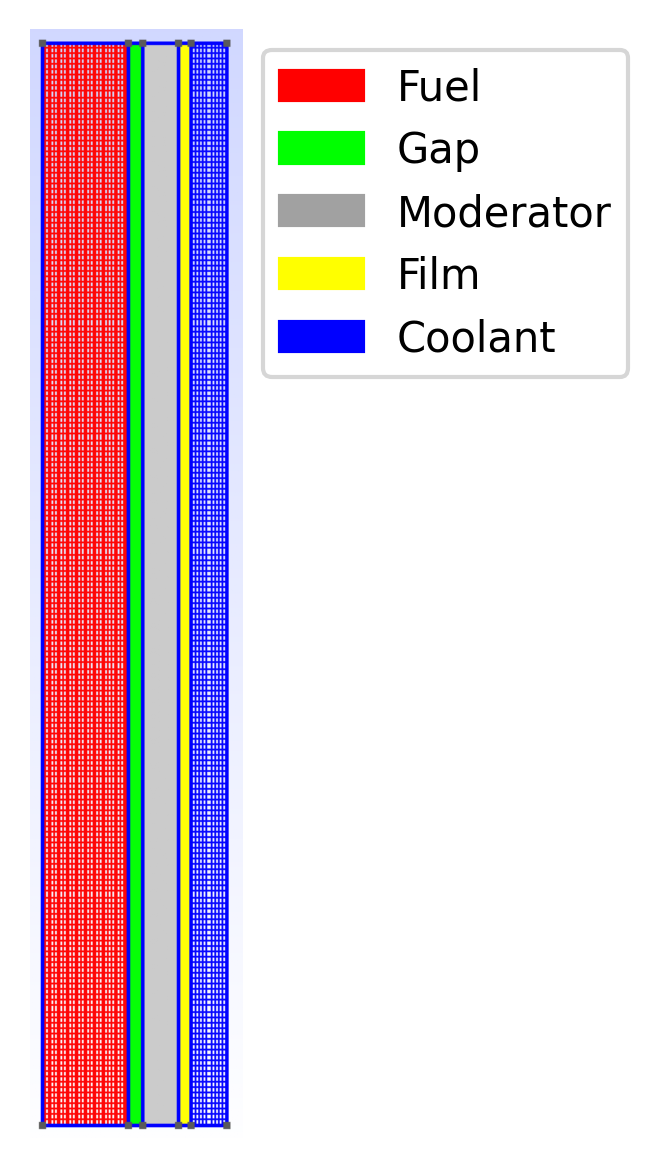
\includegraphics[width=0.45\linewidth]{figures-thermal/2D-preliminar-mesh2}
	\hfill
	\caption{Scaled-down version of the geometry.}
	\label{fig:th-ver-mesh}
\end{figure}

\begin{figure}[htbp!]
	\centering
    \subfloat[Fuel centerline and coolant axial temperatures.]{
        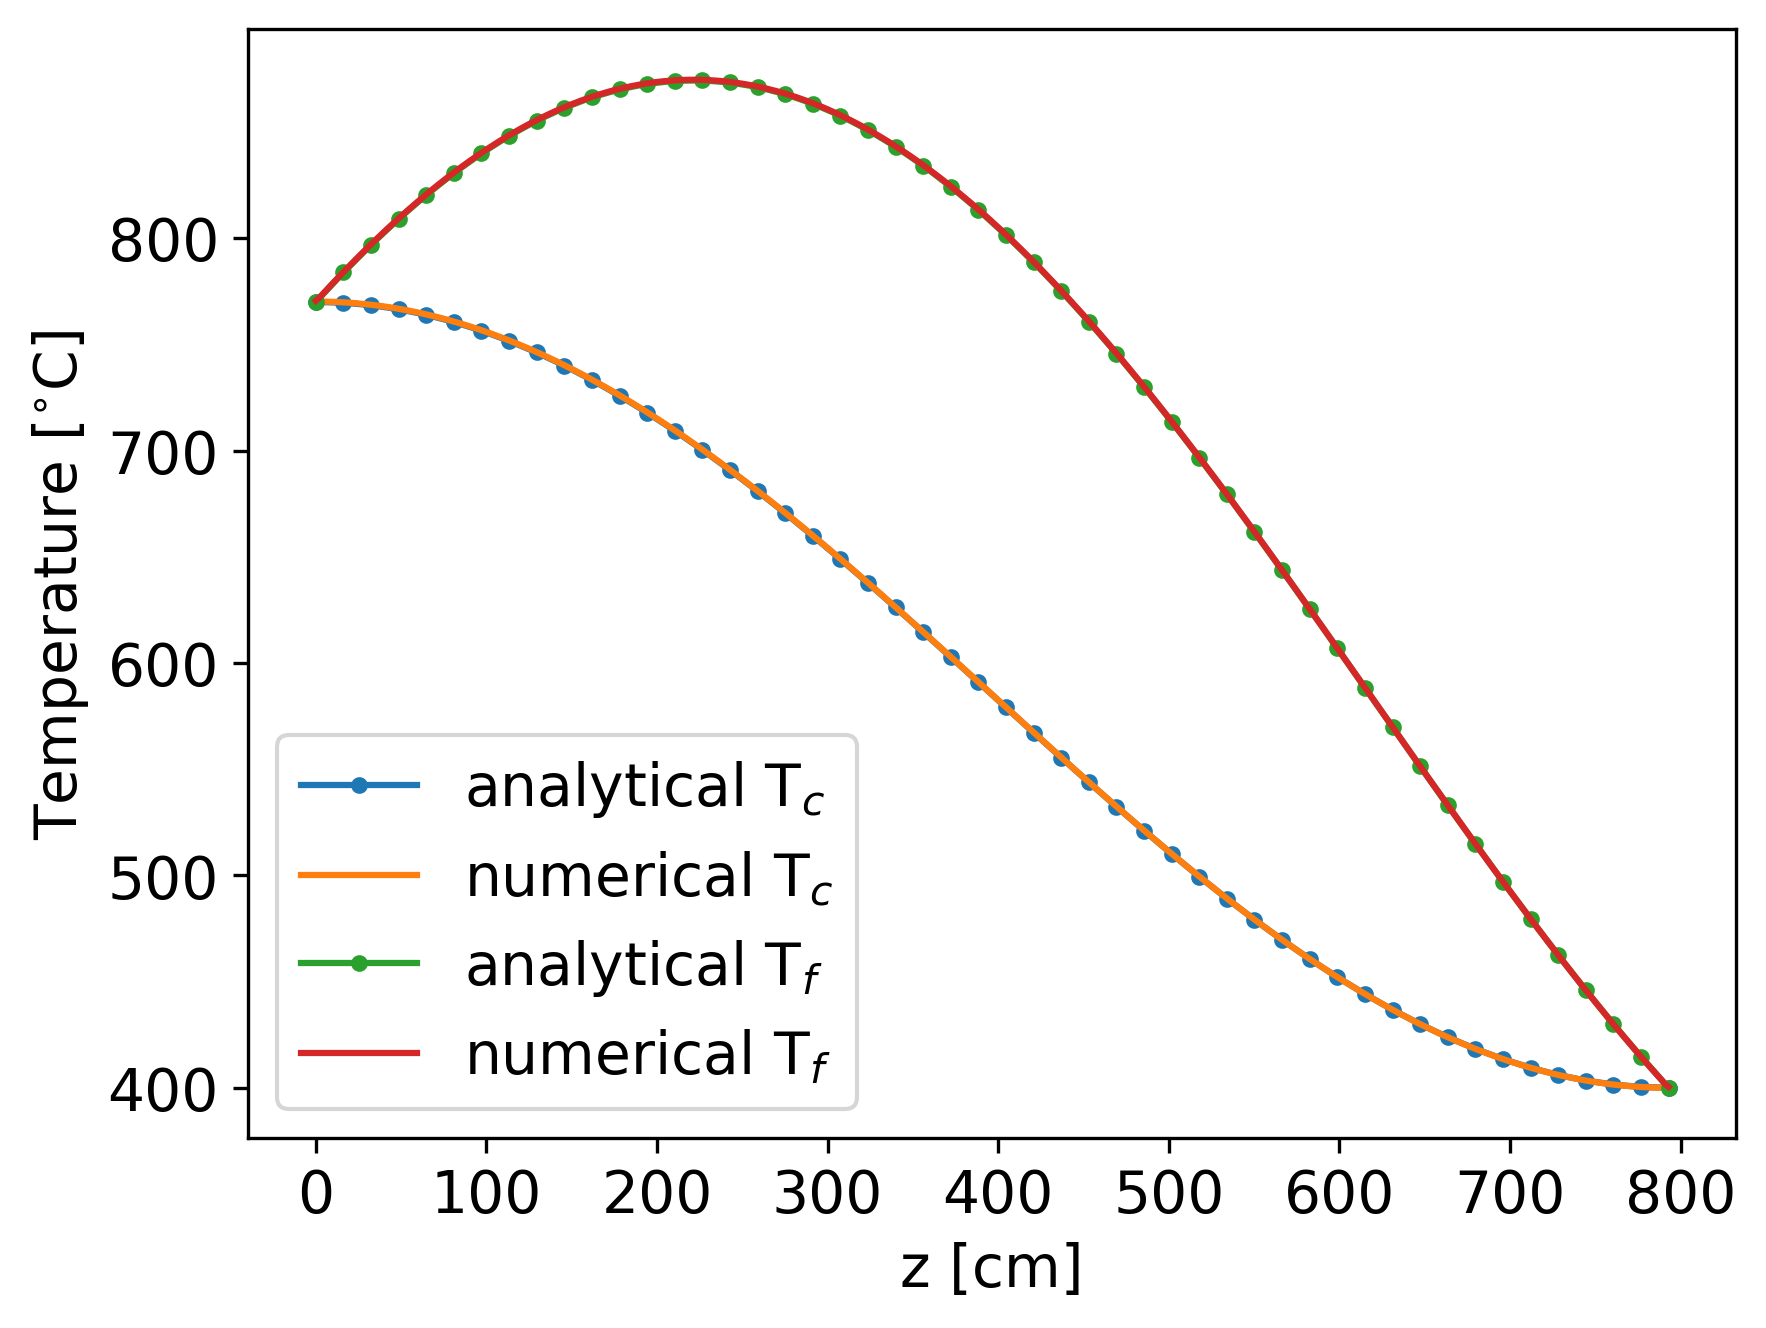
\includegraphics[width=0.45\textwidth]{figures-thermal/2D-preliminar-axial}
    }
    \subfloat[Radial temperature at z=396.5 cm.]{
        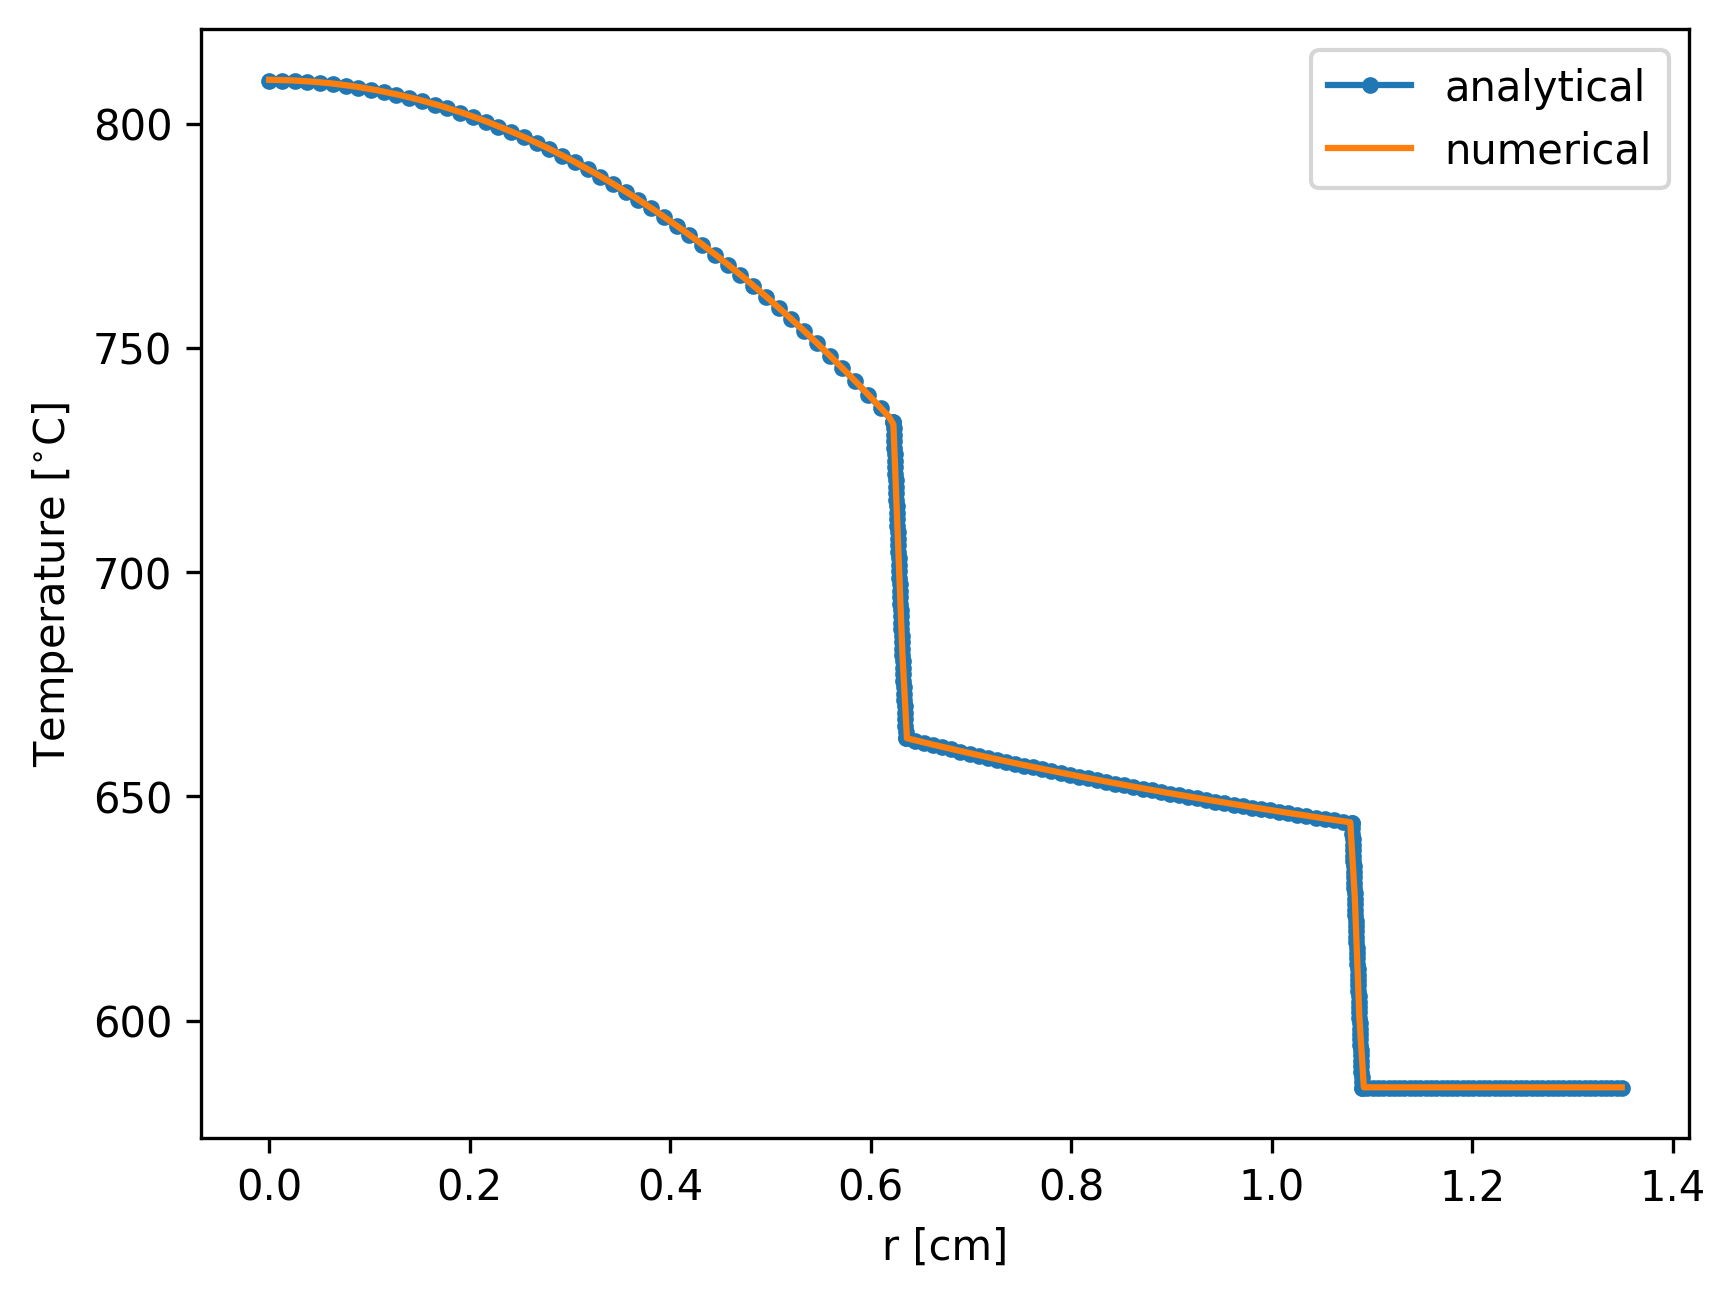
\includegraphics[width=0.45\textwidth]{figures-thermal/2D-preliminar-radial}
    }
	\hfill
    \caption{Temperature profiles.}
	\label{fig:th-ver-results}
\end{figure}

\section{Unit cell problem}

This section will solve the unit cell problem in the hot spot of an HTGR.

\section{Fuel assembly}

This section will calculate the heat profile of a fuel assembly of a HTGR.

\section{Full core}

This section will extend the methodology to a fullcore problem and it will inted to solve Exercise 2 of Phase I of the OECD/NEA MHTGR-350 Benchmark.




\section{Neutronics and Thermal-fluids Coupling}

3 options:
- Heterogeneous model
- Homogenized media and sub-channel unit cell model
- Porous media model

